\documentclass[svgnames, 9pt]{beamer}

\usepackage[utf8]{inputenc}
\usepackage[english]{babel}
\usepackage{amsmath}
\usepackage{amssymb}
\usepackage{xcolor}
\usepackage{graphicx}
\usepackage{tikz}
\usepackage{hyperref}
\usepackage{array}
\usepackage{booktabs}

% ── Color Palette ────────────────────────────────────────────────────────────
\definecolor{maincolor}{RGB}{180, 0, 0}
\definecolor{accentred}{RGB}{220, 50, 50}
\definecolor{lightred}{RGB}{255, 230, 230}
\definecolor{darkgrey}{RGB}{50, 50, 50}
\definecolor{midgrey}{RGB}{120, 120, 120}
\definecolor{codebg}{RGB}{245, 245, 245}

% ── Beamer Theme ─────────────────────────────────────────────────────────────
\mode<presentation>{
    \usetheme{Madrid}
    \usecolortheme[named=maincolor]{structure}

    \setbeamercolor{block title}{bg=maincolor, fg=white}
    \setbeamercolor{block body}{bg=lightred, fg=darkgrey}
    \setbeamercolor{alertblock title}{bg=accentred, fg=white}
    \setbeamercolor{alertblock body}{bg=lightred, fg=darkgrey}
    \setbeamercolor{exampleblock title}{bg=darkgrey, fg=white}
    \setbeamercolor{exampleblock body}{bg=codebg, fg=darkgrey}

    % Compact block padding
    \addtobeamertemplate{block begin}{}{\vspace{-2pt}}
    \addtobeamertemplate{block end}{\vspace{-2pt}}{}
    \addtobeamertemplate{alertblock begin}{}{\vspace{-2pt}}
    \addtobeamertemplate{alertblock end}{\vspace{-2pt}}{}
    \addtobeamertemplate{exampleblock begin}{}{\vspace{-2pt}}
    \addtobeamertemplate{exampleblock end}{\vspace{-2pt}}{}

    % Tighter font sizing
    \setbeamerfont{block title}{size=\footnotesize}
    \setbeamerfont{block body}{size=\footnotesize}
    \setbeamerfont{alertblock title}{size=\footnotesize}
    \setbeamerfont{alertblock body}{size=\footnotesize}
    \setbeamerfont{exampleblock title}{size=\footnotesize}
    \setbeamerfont{exampleblock body}{size=\footnotesize}

    % Footer
    \setbeamertemplate{footline}{%
        \leavevmode%
        \hbox{%
            \begin{beamercolorbox}[wd=.30\paperwidth,ht=2.2ex,dp=1ex,
                leftskip=.3cm plus1fill,rightskip=.3cm]{author in head/foot}%
                \usebeamerfont{author in head/foot}\insertshortauthor
            \end{beamercolorbox}%
            \begin{beamercolorbox}[wd=.25\paperwidth,ht=2.2ex,dp=1ex,
                leftskip=.3cm,rightskip=.3cm plus1fil]{institute in head/foot}%
                \usebeamerfont{institute in head/foot}\insertshortinstitute
            \end{beamercolorbox}%
            \begin{beamercolorbox}[wd=.20\paperwidth,ht=2.2ex,dp=1ex,
                leftskip=.3cm,rightskip=.3cm plus1fil]{date in head/foot}%
                \usebeamerfont{date in head/foot}\insertshortdate
            \end{beamercolorbox}%
            \begin{beamercolorbox}[wd=.25\paperwidth,ht=2.2ex,dp=1ex,
                leftskip=.3cm,rightskip=.3cm plus1fil]{title in head/foot}%
                \usebeamerfont{title in head/foot}\insertshorttitle\hfill
                \insertframenumber\,/\,\inserttotalframenumber\enspace
            \end{beamercolorbox}%
        }%
        \vskip0pt%
    }

    \setbeamertemplate{navigation symbols}{}
    \setbeamertemplate{itemize item}{\color{maincolor}$\blacktriangleright$}
    \setbeamertemplate{itemize subitem}{\color{accentred}$\bullet$}
}

% ── Tighter list spacing globally ─────────────────────────────────────────────
\newlength{\tightitemsep}
\setlength{\tightitemsep}{2pt}
\let\olditemize\itemize
\renewcommand{\itemize}{%
    \olditemize
    \setlength{\itemsep}{\tightitemsep}%
    \setlength{\parskip}{0pt}%
    \setlength{\parsep}{0pt}%
}

% ── Visualization placeholder box ────────────────────────────────────────────
\newcommand{\vizplaceholder}[2]{%
    \begin{tikzpicture}
        \fill[lightred] (0,0) rectangle (\linewidth,#1);
        \draw[maincolor, thick, dashed] (0,0) rectangle (\linewidth,#1);
        \node[text=maincolor, font=\footnotesize\bfseries] at (0.5\linewidth, 0.55*#1)
            {#2};
        \node[text=midgrey, font=\scriptsize] at (0.5\linewidth, 0.35*#1)
            {Insert map screenshot here};
    \end{tikzpicture}%
}

% ── Inline code ──────────────────────────────────────────────────────────────
\newcommand{\code}[1]{{\ttfamily\footnotesize\color{maincolor}#1}}

% ── Metadata ─────────────────────────────────────────────────────────────────
\title[Shadow Fleet Detection]{Shadow Fleet Detection\\[0.2em]Using Big Data \& AIS Streams}
\author[Group Name]{Student 1 \and Student 2 \and Student 3}
\institute[VU Amsterdam]{Vrije Universiteit Amsterdam\\ Big Data Engineering}
\date{March 2026}

% ═════════════════════════════════════════════════════════════════════════════
\begin{document}
% ═════════════════════════════════════════════════════════════════════════════

% ── Slide 1: Title ───────────────────────────────────────────────────────────
\begin{frame}
    \vspace{0.2em}
    \titlepage
    \vspace{-1.5em}
    \begin{center}
        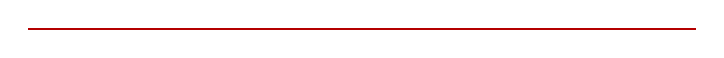
\begin{tikzpicture}
            \fill[maincolor] (0,0) rectangle (0.7\textwidth, 0.03);
        \end{tikzpicture}\\[0.2em]
        {\scriptsize\color{midgrey}
            Detecting dark fleet behaviour from AIS data
            using parallel stream processing}
    \end{center}
    \vfill
\end{frame}

% ── Slide 2: Outline (single, no auto-repeat) ───────────────────────────────
\begin{frame}{Outline}
    \small
    \vspace{0.5em}
    \tableofcontents
    \vfill
\end{frame}

% ═════════════════════════════════════════════════════════════════════════════
\section{Data Streaming, Cleaning \& Chunking}
% ═════════════════════════════════════════════════════════════════════════════

% ── Slide 3: Streaming + Parsing ─────────────────────────────────────────────
\begin{frame}{Pipeline Stage 1 — Streaming \& Cleaning the Data}
    \footnotesize

    AIS data arrives as \textbf{multi-gigabyte CSV files}. The pipeline never
    loads a full file into memory — it reads \textbf{one row at a time} via
    Python generators, cleans each row immediately, and groups valid rows into
    fixed-size \textbf{chunks} that are dispatched to CPU workers.

    \vspace{0.4em}
    \begin{columns}[T]

        \column{0.48\textwidth}
        {\scriptsize\color{maincolor}\textbf{\texttt{reader.py} — Streaming layer}}
        \vspace{0.15em}
        \begin{itemize}\scriptsize
            \item Reads the CSV header \textbf{once} to build a column-index
                  map — field access is O(1) regardless of column order
            \item \texttt{stream\_raw\_rows()} yields one 7-field tuple per
                  row: \textit{timestamp, MMSI, lat, lon, SOG, draught, class}
                  (only 7 of ${\sim}50$ columns are kept)
            \item \texttt{stream\_raw\_rows\_from\_files()} chains \textbf{both
                  input files} into a single continuous row stream — two days
                  of data look like one feed to downstream code
            \item \texttt{stream\_csv\_files\_in\_chunks()} accumulates rows
                  into chunks of $N$ rows and assigns each chunk a global
                  \texttt{chunk\_id} used for ordered merging later
        \end{itemize}

        \column{0.48\textwidth}
        {\scriptsize\color{maincolor}\textbf{\texttt{parser.py} — Cleaning layer}}
        \vspace{0.15em}
        \begin{itemize}\scriptsize
            \item Runs \textbf{inside each worker process}; initialized once
                  per worker to avoid repeated overhead
            \item \texttt{AISRowParser.parse\_row()} applies a \textbf{filter
                  chain} — cheapest checks run first, row dropped on first
                  failure:
            \begin{itemize}\scriptsize
                \item[\color{accentred}$\bullet$] Class A only — drop buoys,
                      aircraft, base stations
                \item[\color{accentred}$\bullet$] Timestamp parseable as UTC
                \item[\color{accentred}$\bullet$] MMSI: 9-digit, not a
                      placeholder (e.g.\ all-zero or all-same digit)
                \item[\color{accentred}$\bullet$] Lat $\in [-90,90]$,
                      Lon $\in [-180,180]$, reject (0,\,0)
                \item[\color{accentred}$\bullet$] SOG and draught parsed as
                      numbers (missing is allowed)
            \end{itemize}
        \end{itemize}

    \end{columns}

    \vspace{0.3em}
    {\scriptsize\color{midgrey}
    \textbf{Outcome:} A 10\,GB file occupies the same RAM as a single chunk
    (${\sim}$thousands of rows). Invalid rows are discarded before they reach
    any anomaly logic. Clean chunks flow into the parallel worker pool.}
\end{frame}

% ═════════════════════════════════════════════════════════════════════════════
\section{Parallel Processing, Merging \& Scoring}
% ═════════════════════════════════════════════════════════════════════════════

% ── Slide 4: Workers + Merge + Scoring ───────────────────────────────────────
\begin{frame}{Pipeline Stage 2 — Workers, Merging \& Scoring}
    \footnotesize

    \begin{columns}[T]

        \column{0.48\textwidth}
        {\scriptsize\color{maincolor}\textbf{\texttt{worker\_pool.py} — Parallel detection}}
        \vspace{0.1em}
        \begin{itemize}\scriptsize
            \item Each chunk is sent to a \textbf{separate CPU worker} via
                  \texttt{Pool.imap\_unordered} — multiple chunks run in
                  parallel simultaneously
            \item Workers are \textbf{initialized once} with port zones and
                  the row parser loaded as process globals (avoids reloading
                  per chunk)
            \item Per chunk, each worker:
            \begin{itemize}\scriptsize
                \item[\color{accentred}$\bullet$] \textbf{Groups} records by
                      MMSI and \textbf{sorts} by timestamp
                \item[\color{accentred}$\bullet$] \textbf{Downsamples} to
                      5-min intervals for anomalies A \& C (reduces noise)
                \item[\color{accentred}$\bullet$] Runs \textbf{Going Dark},
                      \textbf{Draft Change}, \textbf{Teleportation} (D1/D2)
                      rules on consecutive record pairs
                \item[\color{accentred}$\bullet$] Saves \textbf{boundary
                      records} (first + last ping per vessel) for cross-chunk
                      checks
            \end{itemize}
        \end{itemize}

        \column{0.48\textwidth}
        {\scriptsize\color{maincolor}\textbf{\texttt{merge.py} — Cross-chunk stitching}}
        \vspace{0.1em}
        \begin{itemize}\scriptsize
            \item Workers finish \textbf{out of order} — merge layer buffers
                  results and reassembles them by \texttt{chunk\_id}
            \item Compares the \textbf{last record of chunk $N$} with the
                  \textbf{first record of chunk $N\!+\!1$} for the same
                  vessel — catches anomalies that span a chunk boundary
            \item A \& C use downsampled boundary records; D uses
                  full-resolution records
        \end{itemize}

        \vspace{0.3em}
        {\scriptsize\color{maincolor}\textbf{\texttt{run\_detection.py} — Scoring \& output}}
        \vspace{0.1em}
        \begin{itemize}\scriptsize
            \item Aggregates all events per vessel and computes \textbf{DFSI}:
            \vspace{0.1em}

            {\scriptsize
            $\text{DFSI} = \dfrac{\text{max\_gap\_h}}{2}
                         + \dfrac{\text{D2\_jump\_nm}}{10}
                         + \text{draft\_count} \times 15$}

            \vspace{0.15em}
            \item Writes \texttt{dfsi\_results.csv} (all vessels ranked),
                  \texttt{top\_*\_vessel\_map.csv} (map coordinates),
                  \texttt{memory\_profile.csv} (RAM log)
        \end{itemize}

    \end{columns}
\end{frame}

% ═════════════════════════════════════════════════════════════════════════════
\section{Anomaly Detection \& Visualization}
% ═════════════════════════════════════════════════════════════════════════════

% ── Slide 5: Going Dark ─────────────────────────────────────────────────────
\begin{frame}{\footnotesize Anomaly A — Going Dark: AIS Blackout While Moving}
    \begin{columns}[T]

        \column{0.47\textwidth}
        \vspace{0.1em}
        \vizplaceholder{3.6cm}{Going Dark Map}
        \vspace{0.15em}
        {\scriptsize\color{midgrey}
            \textbf{Orange} = last known position \enspace
            \textbf{Purple} = reappearance \enspace
            \textbf{Line} = gap}

        \column{0.50\textwidth}
        {\scriptsize
        \textbf{\color{maincolor}What is it?}\\[2pt]
        Vessel \textbf{switches off AIS transponder}
        while continuing to move, hiding its
        route from authorities.}
        \vspace{0.25em}

        {\scriptsize\textbf{Detection:}}
        \begin{itemize}\scriptsize
            \item Time gap $>$ \textbf{4 hours}
            \item Vessel moved $>$ \textbf{1\,km}
                  (stationary vessels excluded)
            \item Haversine great-circle distance
        \end{itemize}
        \vspace{0.15em}
        {\scriptsize\textbf{Event data stored:}}
        \begin{itemize}\scriptsize
            \item Start/end coords, gap hours, distance
            \item Feeds \code{max\_gap\_h / 2} into DFSI
        \end{itemize}
        \vspace{0.15em}
        {\scriptsize\textbf{Visualization:}}
        \begin{itemize}\scriptsize
            \item Interactive Folium HTML map
            \item Click any dot or line for event details
        \end{itemize}

    \end{columns}
\end{frame}

% ── Slide 6: Teleportation ──────────────────────────────────────────────────
\begin{frame}{\footnotesize Anomaly D — Teleportation: Identity Cloning}
    \begin{columns}[T]

        \column{0.47\textwidth}
        \vspace{0.1em}
        \vizplaceholder{3.6cm}{Teleportation Map}
        \vspace{0.15em}
        {\scriptsize\color{midgrey}
            \textbf{Green} = origin \enspace
            \textbf{Red} = destination \enspace
            \textbf{Blue} = jump}

        \column{0.50\textwidth}
        {\scriptsize
        \textbf{\color{maincolor}What is it?}\\[2pt]
        \textbf{Two ships share the same MMSI.}
        Consecutive pings for one ID appear
        at locations impossible to reach in
        the elapsed time.}
        \vspace{0.25em}

        {\scriptsize\textbf{Detection:}}
        \begin{itemize}\scriptsize
            \item Implied speed
                  $v = d_{\text{nm}} / \Delta t_{\text{h}}$
            \item Flag if $v >$ \textbf{60 knots}
                  (commercial max $\approx$ 30\,kn)
        \end{itemize}
        \vspace{0.15em}
        {\scriptsize\textbf{Event data stored:}}
        \begin{itemize}\scriptsize
            \item Start/end coords, implied speed, distance
            \item Feeds \code{total\_jump\_nm / 10} into DFSI
        \end{itemize}
        \vspace{0.15em}
        {\scriptsize\textbf{Visualization:}}
        \begin{itemize}\scriptsize
            \item Interactive Folium HTML map
            \item Click any dot or line for event details
        \end{itemize}

    \end{columns}
\end{frame}

% ── Slide 7: Future Anomaly (template) ──────────────────────────────────────
\begin{frame}{\footnotesize Anomaly X — [Anomaly Name Here]}
    \begin{columns}[T]

        \column{0.48\textwidth}
        \vspace{0.1em}
        \vizplaceholder{4.5cm}{[Anomaly X] Map}
        \vspace{0.2em}
        {\scriptsize\color{midgrey}
            [Describe dot/line color meanings]}

        \column{0.48\textwidth}
        \begin{block}{\textnormal{What is it?}}
            \scriptsize
            [Describe the suspicious maritime behaviour
            and its relevance to shadow fleet detection.]
        \end{block}
        \vspace{0.15em}
        {\scriptsize\textbf{Detection logic:}}
        \begin{itemize}\scriptsize
            \item [Condition 1 — threshold]
            \item [Condition 2 — constraint]
            \item [Additional filters]
        \end{itemize}
        \vspace{0.15em}
        {\scriptsize\textbf{Event data stored:}}
        \begin{itemize}\scriptsize
            \item [List event fields]
            \item [DFSI contribution]
        \end{itemize}
        \vspace{0.15em}
        {\scriptsize\textbf{Visualization:}}
        \begin{itemize}\scriptsize
            \item [Map type and interaction]
        \end{itemize}

    \end{columns}
\end{frame}

% ── Slide 8: Thank You ──────────────────────────────────────────────────────
\begin{frame}{}
    \vspace{2em}
    \begin{center}
        
\begin{tikzpicture}
            \fill[maincolor] (0,0) rectangle (0.6\textwidth, 0.04);
        \end{tikzpicture}\\[0.6em]
        {\LARGE\color{maincolor}\textbf{Thank you}}\\[0.3em]
        {\small\color{midgrey} Questions \& Discussion}\\[0.6em]
        
\begin{tikzpicture}
            \fill[maincolor] (0,0) rectangle (0.6\textwidth, 0.04);
        \end{tikzpicture}\\[1em]
        {\footnotesize\color{darkgrey}
        \begin{tabular}{r@{\hspace{0.8em}}l}
            \textbf{Repository} & github.com/OnkarBasu/BigdataprojectVU \\[0.2em]
            \textbf{Anomalies}  & A\,(Going Dark),\; C\,(Draft Change),\; D\,(Teleportation) \\[0.2em]
            \textbf{Scoring}    & DFSI --- Dark Fleet Suspicion Index \\
        \end{tabular}}
    \end{center}
\end{frame}

\end{document}
